\subsection{Overview}
In the last years, the concept of "Software Defined Networking"(SDN) got more and more important. The idea of this concept was created by the introduction of the "OpenFlow" protocol in 2008\cite{Mc2008}. This protocol provides a secure communication between switches of a network and some other part of software. Furthermore entries of forwarding tables of these switches can be dynamically modified by this protocol. This allows the ability to change network flows at any time to get an optimal behaviour for special situations. This is basically the idea of "Software Defined Networking", which is currently promoted and propagated by the "Open Networking Foundation".\footnote{https://www.opennetworking.org/about/onf-overview} 

A Software Defined Network contains two important parts. A network with OpenFlow supported switches and a controller. A controller denotes the part of software which controls the behavior of the network at any time by using OpenFlow. In normal networks each switch is its own controller. When a connection starts the switch takes a lookup in its forwarding table to forward the packages. If there is no entry it performs some routing algorithm to get this entry. The problem is that there is nothing which has a view on the whole network. For example if a device has a failure it will take time until each connection node is aware of it. Or maybe if one path of the network is overloaded, it might be faster to send packages via another path. This is a feature, a normal network device can not easily provide. In an emergency case where i.e. a live stream of security cameras needs a higher priority than anything else, a SDN could dynamically provide that in seconds. It works, because a controller of a Software Defined Network sees the network as a graph. It is in a permanent contact with all devices to detect failures. It can get the workload of each switch and can route some communications over other nodes, if a device is overloaded. So the controller can be denoted as the brain of a network and the network nodes as the nerves which follow the orders of the brain. If a new network flow starts, the switch contacts via OpenFlow the controller. The controller decides what to do and sends to the switch a flow table entry. A flow table is the forwarding table in an OpenFlow switch. If the flow finishes, the OpenFlow switch deletes this entry from its flow table. So there is never an uncontrolled flow in the network. The concept of a SDN is visualized in figure \ref{sdn}.\\
\begin{figure}[ht]
\centering
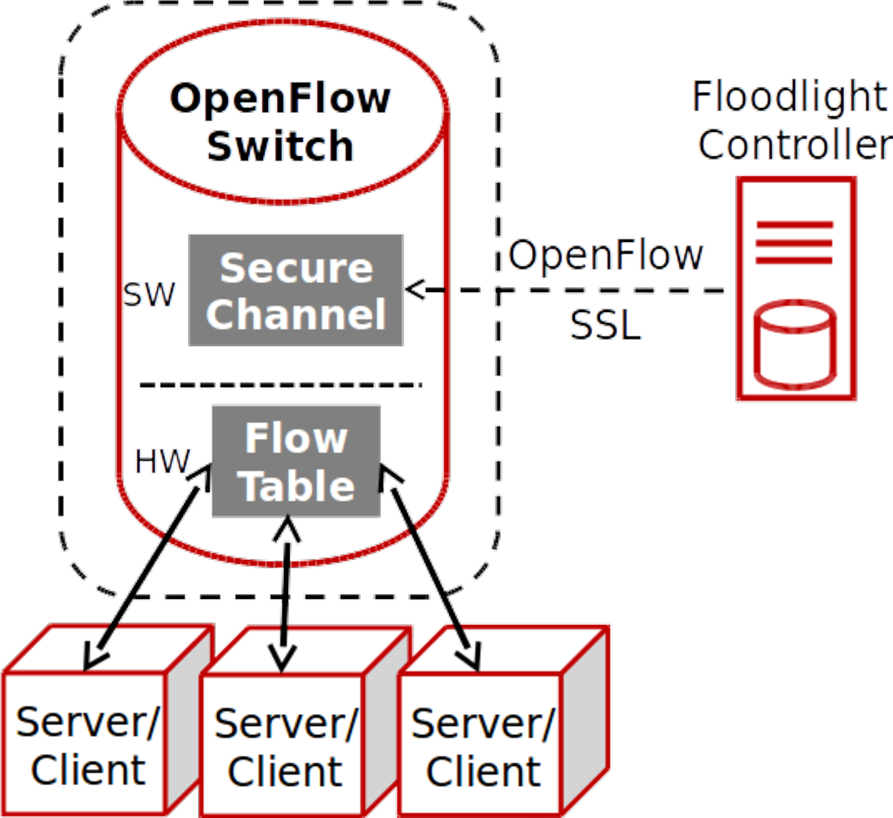
\includegraphics[width=0.25\textwidth]{img/sdn} 

\caption{SDN with Floodlight and Open vSwitch}
\label{sdn}
\end{figure}
 

\subsection{System Setup}
To provide a SDN in the smart Filesystem, the network is organized by the SDN controller Floodlight\cite{flood}. Floodlight is an open source SDN controller, which is written in Java. The fact, that it is written in Java, makes it easy to set it up on many different machines. Floodlight comes with an OpenFlow implementation for virtual switches, as well as physical switches. Moreover it has a lot of additional features. For example features to modify OpenFlow switches or a shortest path routing within a network. Furthermore it is easy to extend Floodlight by using provided interfaces or adding new basic features as so called "Modules". All in all Floodlight allows a quick start in programming a SDN.

As counterpart to the controller, the SDN needs an OpenFlow switch. As told, OpenFlow is a very new protocol. In the moment there are companies like "HP", "Arista", "Brocade" or "Dell" , which build switches with OpenFlow support. Besides that, these companies designing switches for large networks where one switch is expensive. A good alternative to physical switches is the "Open vSwitch" project\footnote{www.openvswitch.org}. With this project it is possible to set up a virtual switch with OpenFlow support on a system, which just behaves like a normal switch. This switch can be controlled by Floodlight very easily. A small disadvantage is, that Open vSwitch is currently supporting OpenFlow 1.0\cite{ovs}, but the latest version is OpenFlow 1.4\cite{ofspec4}. However, version 1.0 supports a lot of features and is sufficient for the needs of the Smart Filesystem.
This Open vSwitch connects all parts of the Smart Filesystem by using OpenVPN connections.     
   
\subsection{Usage in the Smart Filesystem}\label{usage}
In the Smart Filesystem we use Software Defined Networking to measure the file transactions of users within the system. With OpenFlow 1.0, the controller is able to request for flow statistics \cite[P. 31]{ofspec}. These flow statistics contain information such as IP adresses, MAC adresses, used TCP ports, transfered bytes and running time of the flow. With this information the controller is able to tell, that user $u$ with IP $i$ and port $p$ has transferred $x$ bytes in $s$ seconds with an average bandwidth of $x/s$. The identification of the connection with IP and port allows, that more than one user from the same system can use the file system at the same time.

 Of course there are more flows in the file system than just file transfers. But all file transfer flows contain the port $p=50010$ and the IP from one of the datanodes in the HDFS. So if there is a connection, where source or destination is IP $i$ and port $p$, than this is a connection the controller is interested in.
 
 When the controller finds a flow like this, it calculates the bandwidth every five seconds and sends it to the monitoring system. With this data the admins of the file system are able to oversee all transactions and to calculate a very specific power usage for each user. 
 
 \subsection{Implementation and Connection Establishing}               

To establish a connection for file transferring, there are four parts inside the network which need to be done. The first step is shown in figure \ref{nn}.
 
\begin{figure}[ht]
\centering
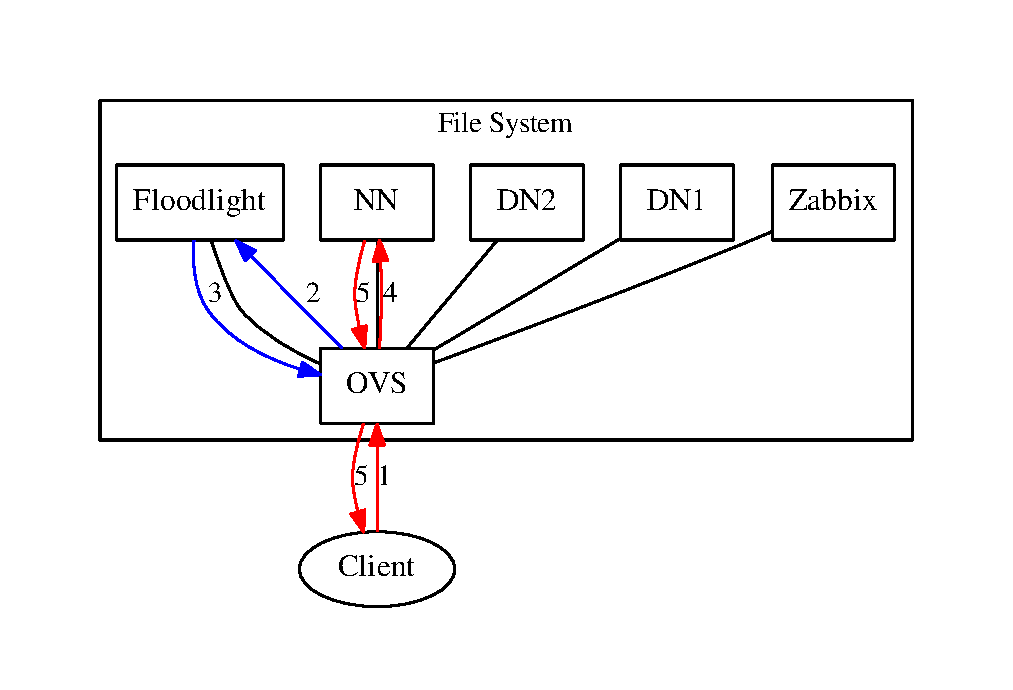
\includegraphics[width=0.5\textwidth]{img/connectionToNamenode} 
\caption{Part 1: A user tries to connect to the Namenode}
\label{nn}
\end{figure}

Figure \ref{nn} shows the internal file system and a client who wants to start a file transfer. The dotted edges denotes client/system interactions and the dashed edges are interactions within the system. The bold edges denotes the openVpn connections of the system.

In step 1 of the figure the client wants to start a file transfer. So the first thing to do is to send a connection request to the system. This request goes firstly to the Open vSwitch(OVS). The switch does not know, where to forward the connection because there is no flow table entry. So the switch asks Floodlight, shown in step 2. In step 3 Floodlight computes the path in the network and sends the flow entry back to the switch. Before a file transfer can start, the Namenode(NN) has to decide on which server the client can connect. So the request goes further to the Namenode, shown in step 4. The Namenode decides for one server and sends these information in step 5 back to the client. Now the client is ready to connect with the Datanode. This interaction is shown in figure \ref{dn}.

\begin{figure}[ht]
\centering
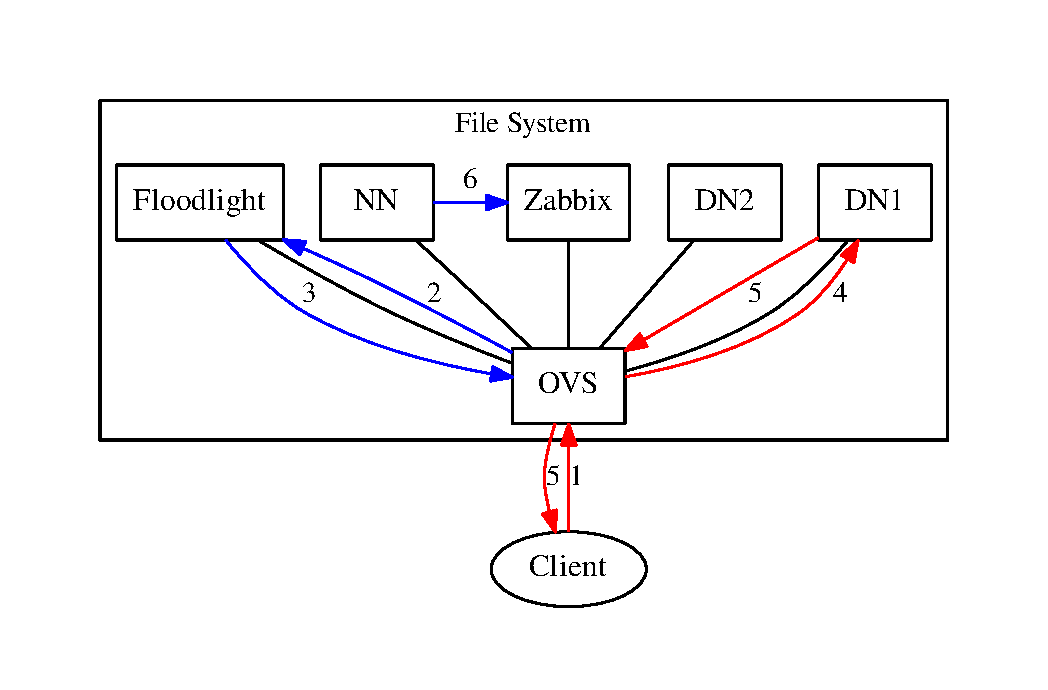
\includegraphics[width=0.5\textwidth]{img/connectionToDatanode} 
\caption{Part 2: Starting connection to the Datanode to begin a file transfer}
\label{dn}
\end{figure}     

In the second part, the client is now really able to start the file transfer and tries to open the connection. Again this connection request stops at the switch, which needs to find out where to forward this request. So the steps 1 till 3 are the same as in the first part. After that, the flow table of the switch contains an entry for this connection request and it can forward it to i.e. Datanode 1(DN1). This is shown in step 4. In step 5 the Datanode answers the request and Client and Datanode 1 start the file transfer. 

Important in the second part is step 6. The Namenode not only decides to which Datanode the connection goes, but also it checks if the client is a registered user. If he is, the Namenode will send the username and the current IP with port of the user to the monitoring system "Zabbix". Why it does that, is described in the third part, which is shown in figure \ref{wc}.    

\begin{figure}[ht]
\centering
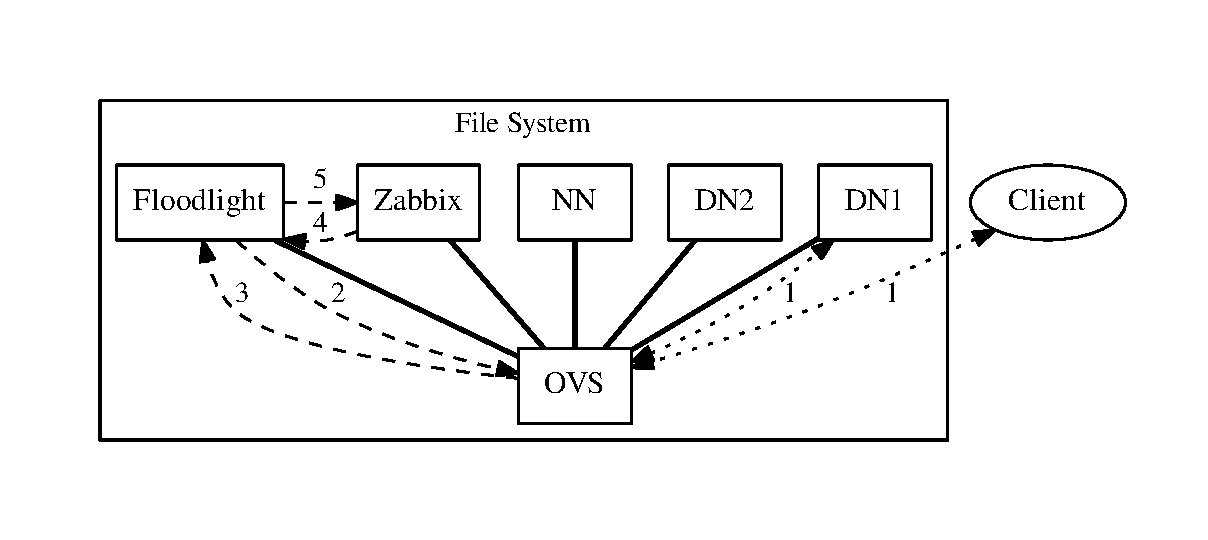
\includegraphics[width=0.5\textwidth]{img/whileConnection} 
\caption{Part 3: While the user is transferring files from or to the Datanode}
\label{wc}
\end{figure}

The figure of part three shows the interactions while a file transfer between client and DN1 is running. Every five seconds Floodlight asks the Open vSwitch for statistics of each entry. Floodlight can do this, because OpenFlow provides a \textit{Read State Message}\cite[p. 30]{ofspec}. With this message, Floodlight gets all the statistics of each flow, which were mention in subsection \ref{usage}. This statistic request is shown in steps two and three. In the moment, there should be two entries for the file transfer. One for uploading and one for downloading. In each case the source/destination is the IP of DN1 with port $50010$. So Floodlight detects, that these are interesting connections and computes the current bandwidth. One problem is, that Floodlight cannot say, which user is using this connection. It only has the IP and port of the user. To solve this problem, the Namenode has sent in the last part the username with corresponding address and port to Zabbix. Now Floodlight can ask Zabbix by using the "Zabbix-API-Client"(\todo{KENNEN WIR DEN SCHON}) which user has the IP and port of the connection. If Zabbix has such an entry, it will send the username to Floodlight, shown in step 4. Now Floodlight can compute the bandwidth for each user and sends it back to Zabbix. This is shown in step 5.

With this procedure, the file system is able to create a precise bandwidth usage for each user every five seconds. After Floodlight has got the connection information from Zabbix, it hashes them to avoid more unnecessary requests. To mention is, that these statistic requests are not bound to the five seconds. This was just a decision to create not too much traffic.

To be sure to get the statistics of the complete flow, the system needs a fourth part, see figure \ref{cc}.  

\begin{figure}[ht]
\centering
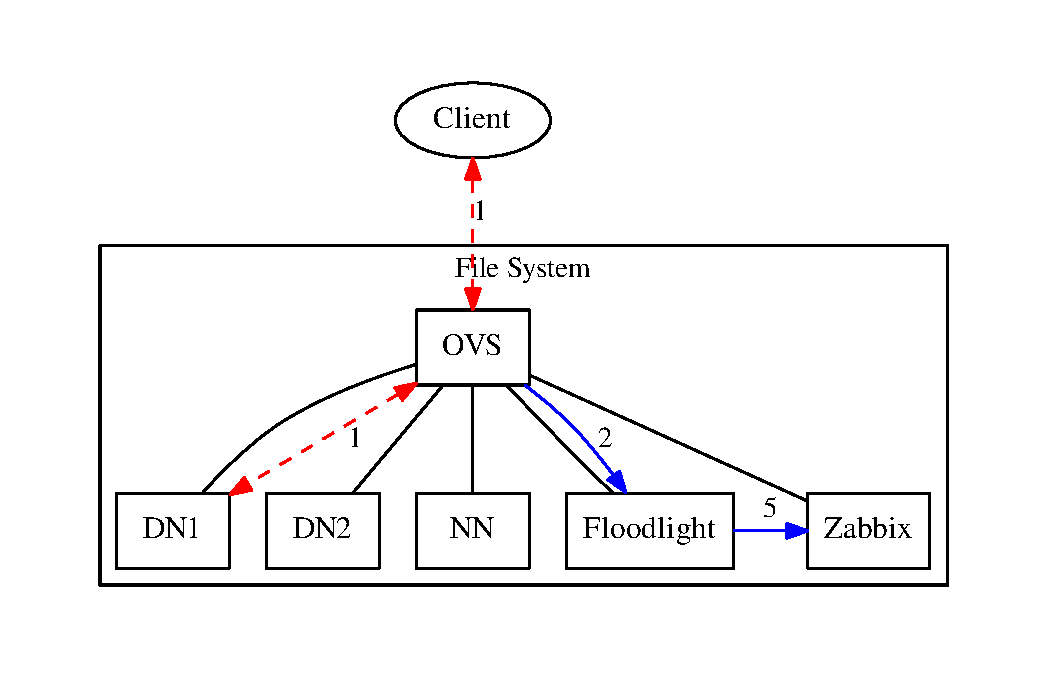
\includegraphics[width=0.5\textwidth]{img/closeConnection} 
\caption{Part 4: Closing connection after file transfer}
\label{cc}
\end{figure}

The last part shows, what to do if a file transfer has finished. The dashed edges of figure \ref{cc} symbols that the connection just closed. When the flow table entry was created it got an "idle timeout"\cite[p. 11]{ofspec}. When there is no data flow any more, the switch waits this idle timeout(here 5 seconds) until it removes the entry from the flow table. Before it removes the entry, it sends a \textit{Flow-Remove-Message}\cite[p. 37]{ofspec} to Floodlight. These messages are just an option which can be set when the entry is created. With this message, Floodlight not only knows that it can remove the flow from its data structures, but also floodlight gets one last time all statistics of this flow. This message is shown in step 4. So Floodlight can compute the bandwidth for the user again and sends it in step 5 to Zabbix. After that it removes the connection information and user name from the data structures and the flow monitoring is done.

\subsection{Additional Information}

Software Defined Networking is an innovation which contains a lot new and interesting features for future networks. The ability to dynamically modifying and reprogramming a network allows a much further improvement of the QoS aspect. But also for the File System it can bring a lot of advantages.

The problem is that the main concern of SDN is to reprogram a network. In our test system there is only one Open vSwitch. So there are not many possibilities to do that. In larger file systems it could be conceivable to transfer all functions of the Namenode to the controller of the SDN. This could save the energy for one device and would be more compact. Moreover, because the controller is always aware of the traffic in the network, it could check if there are datanodes which has not been used in the last time. If there are some, the controller could set to a sleeping mode until there are new traffic for these datanodes. This could save a lot of energy considering that the Asok05 datanode uses $400\ W$ in idle time. It is also possible to modify paths, if a user uses a special profile to get a faster connection of switches or if the user wants to change the profile while doing file transfer. Changing paths can also help for reducing energy costs. The really big switch "HP 12518 AC Switch Chassis" has a maximum power rating of $10700\ W$ \todo{cite}. Of course this is a very big switch and this power usage is only if all components are 100\% in usage. But it shows that network nodes should be factored into the goal of reducing energy usage. In the end it still needs to be calculated if it is better to use just a few nodes or if it is more energy efficient to spread the traffic over the whole network. 

To conclude, in our test system we are able to separate traffic, such that each user can exactly see how much traffic he or she produced. Moreover the file system can collect a lot of statistic values. But to use this values and the whole power of SDN in the way to provide more energy efficiency, it would need a larger test system.  
